\documentclass{report}

\input{preamble}
\input{macros}
\input{letterfonts}

\title{\Huge{Math 120}}
\author{\huge{PSet 7}}
\date{Oct 24 2024}

\begin{document}

\maketitle
\newpage% or \cleardoublepage
% \pdfbookmark[<level>]{<title>}{<dest>}
\pdfbookmark[section]{\contentsname}{toc}
\tableofcontents
\pagebreak

\chapter{}
\section{PSet 7}

\qs{}{
    Evaluate the scalar line integral
    \[
    \int\limits_C (3x + y) \, ds,
    \]
    where \(C\) is the line segment from \((-1, 3)\) to \((4, 2)\).
}

\sol{
   \[ \int\limits_{C} (3x+y) ds \]  
   \[ (-1,3) \quad (4,2) \] 
   \[ f(t) = (1-,3) + t((4,2) - (-1, 3)) \]
   \[ f(t) = (-1,3) + t(5,-1) = \langle -1 + 5t, 3 - t\rangle \]
   \[ x = -1 + 5t \quad y = 3 - t \quad t \in  [0,1] \]
   \[ ds = \sqrt{\left(\frac{dx}{dt}\right)^{2} + \left(\frac{dy}{dt}\right)^{2}} \, dt\]   
   \[ \frac{dx}{dt} = 5 \quad \frac{dy}{dt} = - 1 \]
   \[ ds = \sqrt{5^{2} + (-1)^{2}} \, dt = \sqrt{26} \, dt \]
   \[ 3x + y \Rightarrow 3(-1+5t) + (3-t) \Rightarrow -3 + 15t + 3 - t = 14t \]
   \[ \int_{0}^{1} 14t \sqrt{26} \, dt \Rightarrow \sqrt{26} \int_{0}^{1} 14t \, dt \] 
   \[ \left. 7\sqrt{26}t^{2}\right|_{0}^{1} = 7\sqrt{26}(1)^{2} - 7\sqrt{27}(0)^{2} = 7\sqrt{26} \]     
}

\newpage 

\qs{}{
    In this problem we will sketch part of the argument that a scalar line integral \(\int_C f \, ds\) is independent of the parameterization of \(C\) that we choose to compute the integral. Suppose \(\vec{r}_1(t)\), \(a \leq t \leq b\), and \(\vec{r}_2(t)\), \(c \leq t \leq d\), are two smooth parameterizations of the same smooth curve \(C\). Assuming that both parameterizations are in the same direction it can be shown that \(\vec{r}_2(t) = \vec{r}_1(w(t))\), for some increasing function \(w(t)\) satisfying \(w(c) = a\) and \(w(d) = b\). If this is the case, show that
    \[
    \int_a^b f(\vec{r}_1(t)) \left| \vec{r}_1'(t) \right| \, dt = \int_c^d f(\vec{r}_2(t)) \left| \vec{r}_2'(t) \right| \, dt
    \]
    for any continuous function \(f\).
}

\sol{
    \[ \int\limits_{c} f \, ds \]
    \[ \vec{r_{1}}(t) \quad a \leq t \leq b \]
    \[ \vec{r_{2}}(t) \quad c \leq t \leq d \]
    \[ \vec{r_{2}}(r) = \vec{r_{1}}(w(t)) \quad w(c) = a \quad w(d) = b \] 
    \[ \int_{a}^{b} f(\vec{r_{1}}(t))|\vec{r_{1}}'(t) \, dt = \int_{c}^{d} f(\vec{r_{2}}(t))|\vec{r_{2}}'(t) \, dt \]
    \[ \vec{r_{2}}'(t) = \frac{d}{dt} \vec{r_{2}}(t) = \frac{d}{dt} \vec{r_{1}}(w(t)) = \vec{r_{1}}'(w(t)) w'(t) \]
    \[ |\vec{r_{2}}'(t)| = |\vec{r_{1}}'(w(t)) | \cdot |w'(t)| \] 
    \[ \int_{c}^{d} f(\vec{r_{2}}(t)) |\vec{r_{2}}'(t)| \, dt = \int_{a}^{b} f(\vec{r_{1}}(t)) |\vec{r_{1}}'(w(t))| \cdot |w'(t)| \, dt\]
    \[ w \text{ maps } [c, d] \text{ to } [a,b] \text{, when } t = c \, , s = a \text{, and when } t = d \, , s = b \]
    \[ \int_{a}^{b} f(\vec{r_{1}})(w(t)) |\vec{r_{1}}'(w(t))| \cdot |w(t)| \, dt = \int_{a}^{b} f(\vec{r_{1}}(s))|\vec{r_{1}}'(s)| \, ds \]
    \[ \int_{a}^{b} f(\vec{r_{1}}'(t))|\vec{r_{1}}'(t)| \, dt = \int_{a}^{b} f(r_{1}(s))|\vec{r_{1}}'(s)| \, ds = \int_{c}^{d} f(\vec{r_{2}}(t))|\vec{r_{2}}'(t)| \, dt  \] 
    $\therefore$ the scalar line integral is independent of the parameterization and the equality holds true for any continuous function f          
}

\qs{}{
    Sketch the vector field \(\vec{F}(x, y) = xy \, \hat{\imath} + \frac{1}{2} \, \hat{\jmath} \).
}

\sol{
    \begin{center}
        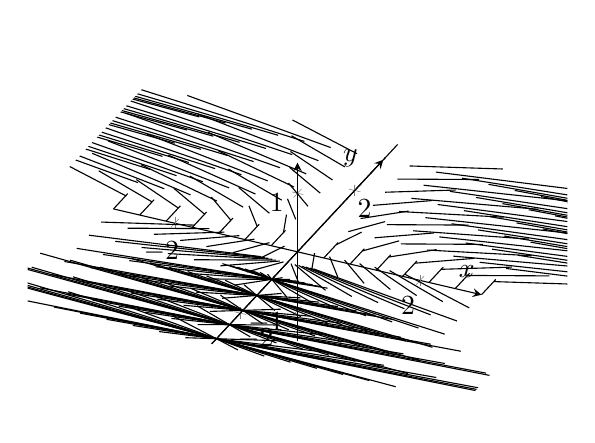
\begin{tikzpicture}
          \begin{axis}[
            axis equal,
            axis lines=middle,
            xmin=-3, xmax=3, ymin=-3, ymax=3,
            xlabel={$x$}, ylabel={$y$},
            samples=15,
            domain=-3:3, y domain=-3:3,
            quiver={
              u={x*y},
              v={0.5},
            },
            every arrow/.append style={-stealth, blue},
          ]
          \addplot3[quiver] {0};
          \end{axis}
        \end{tikzpicture}
    \end{center}
}

\qs{}{
    Given the contour diagram for a function \(f\) shown below, in which dark colors correspond to low values of \(f\) and light colors correspond to high values of \(f\), sketch the gradient vector field \(\vec{F} = \nabla f\).
}

\qs{}{
    A thin wire has the shape of the curve \(C\) parameterized by \(x = \cos t\), \(y = \sin t\), \(z = t\), \(0 \leq t \leq 4\pi\), where \(x, y,\) and \(z\) are measured in centimeters. The linear density of the wire is given by \(\rho(x, y, z) = x^2 z\) grams per centimeter. Find the mass of the wire.
}

\sol{
    \[ x = \cos t \quad y = \sin t \quad z = t \]
    \[ 0 \leq t \leq 4\pi \] 
    \[ \rho(x,y,x) = x^{2}z \frac{\text{grams}}{\text{cm}} \] \
    \[ \text{Mass: } = \int\limits_{C} \rho(x,y,z) ds \] 
    \[ \frac{dx}{dt} = - \sin t \quad \frac{dy}{dt} = \cos t \quad \frac{dz}{dt} = 1 \] 
    \[ ds = \sqrt{\left(\frac{dx}{dt}\right)^{2} + \left(\frac{dy}{dt}\right)^{2} + \left(\frac{dz}{dt}\right)^{2} } \, dt \] 
    \[ ds = \sqrt{\left(-\sin(t)\right)^{2} + \left(\cos (t)\right)^{2} + \left(1\right)^{2} } \, dt \]  
    \[ ds = \sqrt{1 + 1} \, dt = \sqrt{2} \, dt \] 
    \[ \rho(x,y,z) = x^{2}z \Rightarrow \cos^{2}t \cdot t \Rightarrow t \cos^{2} t \]
    \[ \text{Mass: } \int_{0}^{4\pi} \rho(t) ds = \int_{0}^{4\pi} t \cos^{2} t \sqrt{2} \, dt \]
    \[ \sqrt{2} \int_{0}^{4} t \cos ^{2} t dt \quad \cos^{2}t = \frac{1 + \cos 2t}{2} \] 
    \[ \sqrt{2} \int_{0}^{4\pi} t \left(\frac{1 + \cos 2t}{2}\right) \, dt \Rightarrow \frac{\sqrt{2}}{2} \int_{0}^{4\pi} t (1 + \cos 2t )\, dt \]
    \[ \frac{\sqrt{2}}{2} \int_{0}^{4\pi} t \, dt + \frac{\sqrt{2}}{2} \int_{0}^{4\pi} t \cos 2t \, dt \] 
    \[ \int_{0}^{4\pi} t \, dt = \left. \frac{t^{2}}{2}\right|_{0}^{4\pi} \Rightarrow \frac{\sqrt{2}}{2} \frac{16 \pi^{2}}{2} - \frac{\sqrt{2}}{2} \frac{0}{2} = 4\sqrt{2}\pi^{2} \] 
    \[ u = t \quad du = dt \]
    \[ v = \frac{1}{2} \sin 2t \quad dv = \cos 2t \]
    \[ \int t \cos 2t \, dt = t \cdot \frac{1}{2} \sin 2t - \int \frac{1}{2} \sin 2t dt = \frac{1}{2} t \sin 2t + \frac{1}{4} \cos 2t + k \]
    \[ \left[ \frac{1}{2} t \sin 2t + \frac{1}{4} \cos 2t \right]_{0}^{4 \pi} = \left( \frac{1}{2} \cdot 4 \pi \cdot 0 + \frac{1}{4} \cdot 1 \right) - \left(0 + \frac{1}{4} \cdot 1\right) = 0 \]
    \[ 4 \sqrt{2} \pi^{2} + 0 = 4 \sqrt{2}\pi^{2} \]       
}

\qs{}{
    Let \(\vec{F}\) be the vector field shown below, and let \(C\) be the unit circle, oriented clockwise. Is the vector line integral
    \[
    \int_C \vec{F} \cdot d\vec{r}
    \]
    positive, negative, or zero? Explain your reasoning.
}

\qs{}{
    Evaluate the line integral 
    \[
    \int_C \sin x \, dx + \cos y \, dy
    \]
    where \(C\) consists of the top half of the circle \(x^2 + y^2 = 1\) from \((1, 0)\) to \((-1, 0)\) and the line segment from \((-1, 0)\) to \((-2, 3)\). (Remember that when you see an integral that looks like 
    \[
    \int_C P(x, y) \, dx + \int_C Q(x, y) \, dy
    \]
    it is a shorthand notation for 
    \[
    \int_C \vec{F}(\vec{r}(t)) \cdot d\vec{r}
    \]
    where \(\vec{F}(x, y) = \langle P(x, y), Q(x, y) \rangle\). The analogous thing is true in three dimensions.)
}

\sol{
    \[ x^{2} + y^{2} = 1 \quad x = \cos t \quad y = \sin t \quad t \in [0, \pi] \]
    \[ x(t) = (1 - t)(-1) + t(-2) \quad y(t) = (1 - t)(0) + t(3) \quad t \in [0,1] \] 
    \[ \vec{F}(x,y) = \langle \sin x, \cos y \rangle \]
    \[ \int\limits_{C} \sin x \cos y \, dy \] 
    \[ \frac{dx}{dt} = -\sin t \, dt \quad \frac{dy}{dt} = \cos t \, dt \]
    \[ \int\limits_{C_{1}} \cos x + \sin y \, dy = \int_{0}^{\pi} \sin (\cos t)(-\sin t) \, dt + \cos(\sin t) \cos t \, dt \]
    \[ x(t) = -1 - t \quad y(t) = 3t \quad t \in [0,1] \]     
}

\qs{}{
    Compute the line integral of the vector field 
    \[
    \vec{F}(x, y) = \frac{x}{\sqrt{x^2 + y^2}} \hat{\imath} + \frac{y}{\sqrt{x^2 + y^2}} \hat{\jmath}
    \]
    along the parabola \(x = 1 + y^2\) from \((2, -1)\) to \((2, 1)\).
}

\qs{}{
    Evaluate the line integral of the vector field
    \[
    \vec{F}(x, y, z) = (x + y) \hat{\imath} + (y - z) \hat{\jmath} + z^2 \hat{k}
    \]
    along the path parameterized by 
    \[
    \vec{r}(t) = t^2 \hat{\imath} + t^3 \hat{\jmath} + t^2 \hat{k}, \quad 0 \leq t \leq 1.
    \]
}

\qs{}{
    For each of the following vector fields \(\vec{F}\) and curves \(C\), find a function \(f\) such that \(\vec{F} = \nabla f\) and use this function to evaluate 
    \[
    \int_C \vec{F} \cdot d\vec{r}
    \]
    along the given directed curve \(C\).
    \begin{enumerate}
        \item \(\vec{F}(x, y) = \langle x^2, y^2 \rangle\),  
        \(C\) is the arc of the parabola \(y = 2x^2\) from \((-1, 2)\) to \((2, 8)\).

        \item \(\vec{F}(x, y, z) = \langle e^y, xe^y, (z + 1)e^z \rangle\),  
        \(C : \vec{r}(t) = \langle t, t^2, t^3 \rangle\), \(0 \leq t \leq 1\).
    \end{enumerate}
}

\qs{}{
    Clairaut’s Theorem implies that if the vector field \(\vec{F} = P \hat{\imath} + Q \hat{\jmath} + R \hat{k}\) is conservative and \(P, Q,\) and \(R\) have continuous first-order partial derivatives, then
    \[
    \frac{\partial P}{\partial y} = \frac{\partial Q}{\partial x}, \quad 
    \frac{\partial P}{\partial z} = \frac{\partial R}{\partial x}, \quad 
    \frac{\partial Q}{\partial z} = \frac{\partial R}{\partial y}.
    \]
    \begin{enumerate}
        \item Use the statement above to show that the vector line integral
        \[
        \int_C x \, dx + 2x \, dy + xz \, dz
        \]
        is not independent of path.

        \item Find two directed curves \(C_1\) and \(C_2\) that start at the same point and end at the same point, such that
        \[
        \int_{C_1} x \, dx + 2x \, dy + xz \, dz \neq \int_{C_2} x \, dx + 2x \, dy + xz \, dz.
        \]
    \end{enumerate}
}

\qs{}{
    The force exerted by an electric charge at the origin on a charged particle at a point \((x, y, z)\) with position vector \(\vec{r} = \langle x, y, z \rangle\) is 
    \[
    \vec{F}(\vec{r}) = K \frac{\vec{r}}{|\vec{r}|^3},
    \]
    where \(K\) is a constant. Find the work done on the particle as it moves along the straight line from \((0, 3, 0)\) to \((1, 3, 2)\) in two ways:
    \begin{enumerate}
        \item Parameterize the line segment, and compute 
        \[
        \int_a^b \vec{F}(\vec{r}(t)) \cdot \vec{r}'(t) \, dt
        \]
        directly.
        
        \item Although \(\vec{F}\) is not defined at the origin, it turns out that \(\vec{F}\) is conservative on its domain. Find a potential function \(f\), and use the Fundamental Theorem of Line Integrals to compute the work done on the particle.
    \end{enumerate}
}

\end{document}